In the facial expression recognition task, unlike other problems' datasets such as ImageNet~\cite{krizhevsky2012imagenet}, the available datasets are usually small and unbalanced, providing only a few examples to some emotion categories, making neural networks hard to train. Below we describe briefly the datasets that are used in our analysis.

\section{FER+}
The Facial Expression Recognition 2013 (FER2013) dataset, which was introduced in the ICML 2013 Challenges in Representation Learning~\cite{tang2013challenges}, was created by Google image search API. The dataset consists of 48-by-48 pixel grayscale images of human faces annotated with the seven basic emotions (neutral, happiness, surprise, sadness, anger, disgust, and fear). The label accuracy of this dataset is not very high, and as a result a newer version of this dataset called FER+ has been released by Microsoft~\cite{barsoum2016training}, where each image has been labeled by 10 crowd-sourced taggers, which provide better ground truth labels than the original FER labels. Figure~\ref{fig:FERPLUS_FER} shows some examples of images with labels from the initial dataset(FER2013) and the newer version(FER+).

\begin{figure}[]
    \begin{center}
    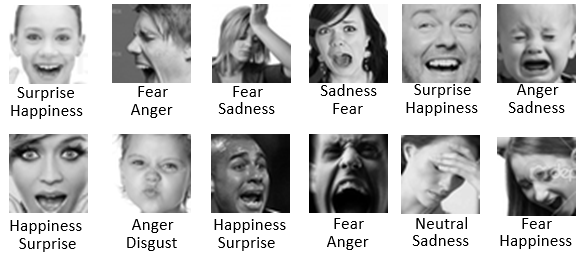
\includegraphics[width=0.6\textwidth]{images/FERPLUS_FER.png}
    \end{center}
    \caption{FER vs FER+ examples. Top labels are FER and bottom labels are FER+ (after majority voting). Figure taken from~\cite{barsoum2016training}.} \label{fig:FERPLUS_FER}
\end{figure}

 The FER+ dataset includes the label contempt to the list of possible emotions. Finally, the resulting dataset contains 28,709 images in training set, 3,589 images in validation set, and 3,589 images in test set. See Figure~\ref{fig:ferplus} for examples from the dataset with their corresponding emotion. 
 
 \begin{figure}[]
    \begin{center}
    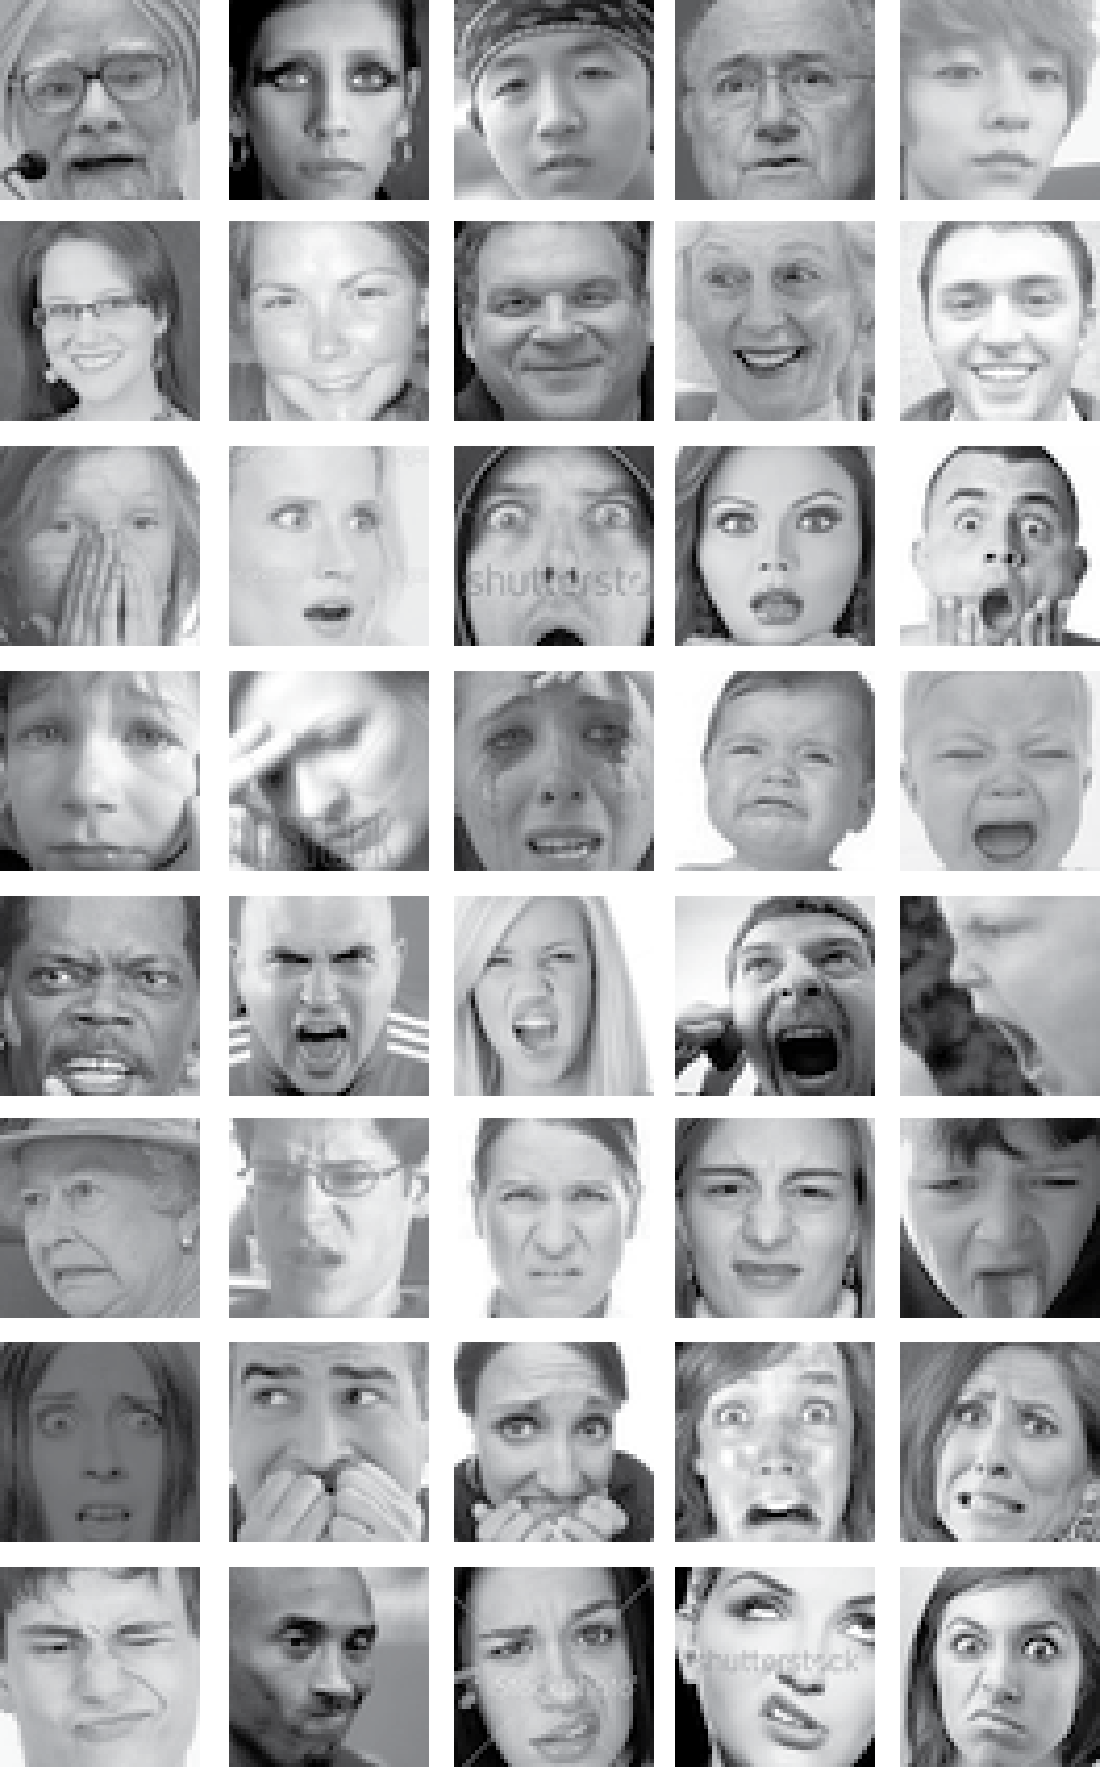
\includegraphics[width=0.8\textwidth]{images/ferplus.png}
    \end{center}
    \caption{Examples of the Fer+ dataset. Each row consists of faces of the same emotion, starting from top row: neutral, happiness, surprise, sadness, anger, disgust, fear, and contempt.} \label{fig:ferplus}
\end{figure}

\section{Extended Cohn-Kanade (CK+)}
The extended Cohn-Kanade (CK+) database consists of 593 sequences across 123 persons which are FACS coded at the peak frame. All sequences start from the neutral face and end to the peak expression. So for each sequence of images there is only 1 file with the Action Units. From those 593 sequences, 327 have emotion labels from 7 basic emotions (anger, contempt, disgust, fear, happy, sadness, surprise). See Figure~\ref{fig:Cohn_kanade} for examples from the dataset with their corresponding emotion and their action units. Also Table~\ref{tab:AU} depicts the action units along with their description and their connection with the basic emotional states that are used to our experiments.

 \begin{figure}[H]
    \begin{center}
    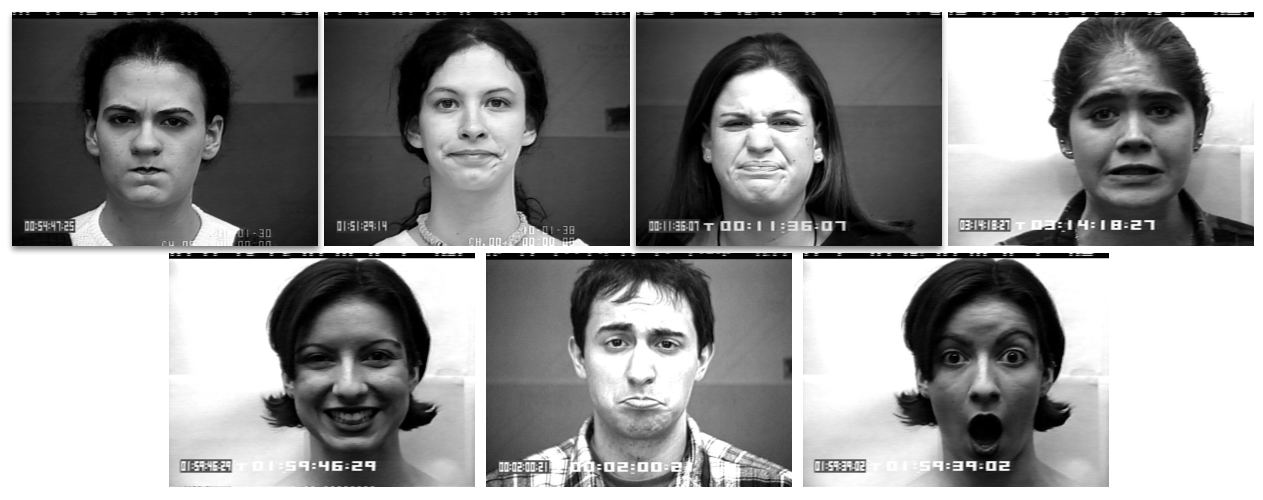
\includegraphics[width=0.6 \textwidth]{images/Cohn_kanade.pdf}
    \end{center}
    \caption{Examples of the CK+ dataset. From left to right: (a) Anger AU 4, 7, 17, 23, 24, (b) Contempt AU 14, 15, 24, (c) Disgust AU 9, 15, 17, 24, (d) Fear AU 1, 4, 7, 20, 25, (e) Happy AU 6, 12, 16, 25, (f) Sadness AU 1, 2, 4, 15, 17, (g) Surprise AU 1, 2, 5, 25, 27} \label{fig:Cohn_kanade}
\end{figure}

\begin{table}[]
\centering
\begin{tabular}{c|c|c}
\hline
\textbf{AU} & \textbf{Name}        & \textbf{Associated emotions}     \\ \hline
1           & Inner Brow Raiser    & Surprise, Sadness, Disgust, Fear \\ \hline
2           & Outer Brow Raiser    & Surprise, Sadness, Fear          \\ \hline
4           & Brow Lowerer         & Sadness, Anger, Disgust, Fear    \\ \hline
5           & Upper Lip Raiser     & Surprise, Anger, Fear            \\ \hline
6           & Cheek Raiser         & Happiness, Sadness               \\ \hline
7           & Lid Tightener        & Fear                             \\ \hline
9           & Nose Wrinkler        & Disgust                          \\ \hline
10          & Upper Lip Raiser     & Disgust                          \\ \hline
11          & Nasolabial Deepener  & -                                \\ \hline
12          & Lip Corner Puller    & Happiness                        \\ \hline
13          & Check Puller         & -                                \\ \hline
14          & Dimpler              & Contempt                         \\ \hline
15          & Lip Corner Depressor & Sadness, Anger, Disgust          \\ \hline
16          & Lower Lip Depressor  & -                                \\ \hline
17          & Chin Raiser          & Sadness, Anger, Disgust          \\ \hline
18          & Lip Puckerer         & -                                \\ \hline
20          & Lip Stretcher        & Fear                             \\ \hline
21          & Neck Tightener       & -                                \\ \hline
23          & Lip Tightener        & Anger                            \\ \hline
24          & Lip Pressor          & -                                \\ \hline
25          & Lips Part            & Happiness, Surprise              \\ \hline
26          & Jaw Drop             & -                                \\ \hline
27          & Mouth Stretch        & -                                \\ \hline
28          & Lip Suck             & -                                \\ \hline
29          & Jaw Thrust           & -                                \\ \hline
31          & Jaw Clencher         & -                                \\ \hline
34          & Cheek Puff           & -                                \\ \hline
38          & Nostril Dilator      & -                                \\ \hline
39          & Nostril Compressor   & -                                \\ \hline
43          & Eyes Closed          & -                                \\ \hline
\end{tabular}
\caption{Action unit codes with their description and their association with basic emotional states.}
\label{tab:AU}
\end{table}

\section{IMDB-WIKI 500+}
Also we use the IMDB-WIKI dataset, the largest publicly available dataset of face images annotated with age and gender~\cite{rothe2015dex}. The dataset contains 460,723 face images from 20,284 celebrities from IMDB, and 62,328 from Wikipedia. A few examples are given in Figure~\ref{fig:wiki}.

 \begin{figure}[H]
    \begin{center}
    
\includegraphics[width=0.6\textwidth]{images/wiki.png}
    \end{center}
    \caption{Examples of the IMDB-WIKI dataset.} \label{fig:wiki}
\end{figure}

\begin{table}[H]
\centering
\begin{tabular}{c|c|c|c|c|c|c|c|c|}
\cline{2-9}
                                       & \textbf{NE} & \textbf{HA} & \textbf{SU} & \textbf{SA} & \textbf{AN} & \textbf{DI} & \textbf{FE} & \textbf{CO} \\ \hline
\multicolumn{1}{|c|}{\textbf{FER2013}} & 6198        & 8989        & 4002        & 6077        & 4953        & 547         & 5121        & 0           \\ \hline
\multicolumn{1}{|c|}{\textbf{FER+}}    & 11660       & 9318        & 4377        & 4746        & 3244        & 303         & 1023        & 291         \\ \hline
\multicolumn{1}{|c|}{\textbf{CK+}}     & 0           & 69          & 83          & 28          & 45          & 59          & 25          & 18          \\ \hline
\end{tabular}
\caption{Number of faces per emotion for each dataset. NE: Neutral, HA: Happiness, SU: Surprise, SA: Sadness, AN: Anger, DI: Disgust, FE: Fear, CO: Contempt}
\label{tab:datasets}
\end{table}


%\afterpage{\blankpage}